% vim: ts=2:sw=2:tw=80:et
This manual describes the use and operation of Arbwave, the arbitrary waveform
experimental control program.

\section{What is Arbwave?\index{What is Arbwave?}}

\section{What can Arbwave do?}

We can also refer to a figure as Fig.~\ref{fig:intro:jdk_grid_example}.

\begin{figure}[hb]
    \centerline{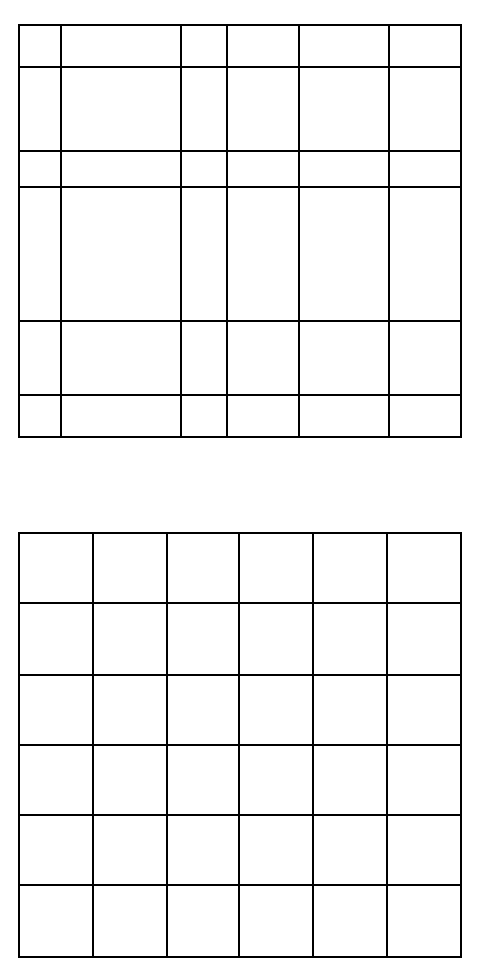
\includegraphics[angle=-90]{figures/jdk_grid_example}}
    \caption{Regular mesh on the left; stretched mesh, in both directions, on
             the right.} 
    \label{fig:intro:jdk_grid_example}
\end{figure}

We just love to cite \citet{Rambo:1989}.


\section{Supported Hardware}\label{sec:hardware}
\begin{center}
\tablefirsthead{%
  \hline
  \textbf{\large Manufacturer} &
  \textbf{\large Model} &
  \textbf{\large Description} &
  \textbf{\large Supported Driver} \\
  \hline
  \hline
}
\tablehead{%
  \hline
  \multicolumn{4}{|l|}{\small\sl continued from previous page}\\
  \hline
  \textbf{\large Manufacturer} &
  \textbf{\large Model} &
  \textbf{\large Description} &
  \textbf{\large Supported Driver} \\
  \hline
  \hline
}
\tabletail{%
  \hline
  \multicolumn{4}{|r|}{\small\sl continued on next page}\\
  \hline
}
\tablelasttail{\hline}
\bottomcaption{Supported Hardware}
%
%
\begin{supertabular}{|l|c|l|r|}
  NI & PCI-6221 & 16-bit Analog output, n-channel & NiDAQmx \\
     &          &                                 & comedi (in progress) \\
  NI & PCI-6225 & 16-bit Analog output, n-channel & NiDAQmx \\
     &          &                                 & comedi (in progress) \\
  NI & PCI-6229 & 16-bit Analog output, n-channel & NiDAQmx \\
     &          &                                 & comedi (in progress) \\
  NI & PCI-6723 & 12-bit Analog output, 32-channel & NiDAQmx \\
     &          &                                 & comedi (in progress) \\
  NI & PCI-6733 & 16-bit Analog output, 8-channel & NiDAQmx \\
     &          &                                 & comedi (in progress) \\
  NI & PXI-6733 & 16-bit Analog output, 8-channel & NiDAQmx \\
     &          &                                 & comedi (in progress) \\
  Viewpoint & DIO-64 & Digital input/output, 64-channel & DIO64 \\
  Marvin Test & GX164x & 16-bit Analog output, 64-channel & GxAo (in progress) \\
  Marvin Test & GX3500 & FPGA based digital output, 120-channel & GxFpga \\
\end{supertabular}
\end{center}
